\documentclass[lmodern, utf8, zavrsni]{fit}

%\batchmode
%\usepackage{booktabs}
\usepackage{listings}
\usepackage{longtable}
\usepackage{xcolor}
\usepackage{float}
\usepackage{enumitem}
\usepackage{hyperref}
\usepackage{enumerate}
\usepackage{graphicx}
\usepackage{etoolbox}
\usepackage{datetime}
\usepackage{needspace}
\usepackage{titlesec}
\usepackage{footnote}
%\titleformat{\chapter}[display]{\normalfont\huge\bfseries}{\chaptertitlename\ \thechapter}{20pt}{\Huge}

\begin{document}

\widowpenalty=300
\clubpenalty=300
\setlength{\parindent}{0pt}

\lstset{
  language=bash,
  backgroundcolor=\color{gray!25},
  basicstyle=\ttfamily \footnotesize,
  breaklines=true,
  prebreak=\raisebox{0ex}[0ex][0ex] {\ensuremath{\hookleftarrow}},
  columns=fullflexible,
  keywords={},
  mathescape=false
}


% this alters "before" spacing (the second length argument) to 0
%\titlespacing*{\chapter}{0pt}{0pt}{40pt}

% this changes "before" spacing back to its default of 50pt
%\titlespacing*{\chapter}{0pt}{50pt}{40pt}}

%\titlespacing*{\chapter}{0pt}{-50pt}{18pt}
%\titleformat{\chapter}[display]{\normalfont\huge\bfseries}{\chaptertitlename\ \thechapter}{20pt}{\Huge}

\title{Agilni \emph{software development}\newline \color{red}{(Nacrt)}}

\author{Ernad Husremović}
\brindex{DL 2792}
\verzija {0.0.5}
\thesisnumber{9999}
\mentor{mr. Adil Joldić}

\maketitle

\tableofcontents

%\listoftables
%\listoffigures
\newpage

% abstract begin
%\begin{abstract}
%
%To be done 
%
%\keywords{open source software, OSS, Bosna i Hercegovina}
%\end{abstract}

% abstract end

\chapter{Uvod}
\vspace*{-0.7cm}

Šta znači `biti agilan'?

Agilni razvoj software-a ne predstavlja specifični proces. Agilni razvoj je način na koji se razmišlja o razvoju software-a\citep[str. 9]{agileart}.

Osnovna polazišta ovog pristupa opisuje "Agilni manifest"\footnote{\url{http://agilemanifesto.org/iso/en/principles.html}}, koji je definisan kroz četiri vrijednosti i 12 principa:

Vrijednosti:
\begin{itemize}
\item Ljudi i interakcije ispred procesa i softverskih alata
\item \emph{Software} koji funkcioniše ispred detaljne dokumentacije
\item Komunikacija sa klijentima ispred pregovora
\item Odgovor na promjene ispred slijeđenja plana
\end{itemize}

Principi:
\begin{itemize}
\item Glavni prioritet je zadovoljiti zahtjeve klijente kroz ranu i kontinuiranu \emph{isporuku} software-a
\item Blagonaklono prihvatiti \emph{promjene} funkcionalnih zahtjeva, čak i u kasnijim fazama razvoja.
\item Funkcionalan software treba isporučivati \emph{često}, nakon par hefti ili mjeseci, nastojeći da taj period bude što kraći.
\item Najefikasniji način razmejene informacija unutar razvojnog tima je direktna - `face-to-face' komunikacija.
\item Software koji \emph{funkcioniše} je primarna mjera uspjeha projekta.
\item Agilni procesi promoviraju održivi razvoj. Finansijeri, developeri i korisnici trebaju biti u stalnoj koordinaciji, bez obzira na dužinu trajanja projekta.
\item Kontinuirano pažnja na \emph{kvalitet} tehničkih operacije i dobar dizajn povećava agilnost.
\item \emph{Jednostavnost}, kao vještina postizanja maksimalnog učinka sa što manje rada, je krucijalni agilni princip.
\item Najbolja arhitektura, funkcionalni zahtjevi i dizajn se postižu u \emph{samo-organizovanim} timovima.
\item Tim redovno analizira predhodne operacije u cilju bolje efektivnosti (\emph{refleksija}). Na osnovu tih rezultata, tim utvrđuje buduće operacije.
\end{itemize}

\section{Agilne metode}

Najpoznatije Agilne metode\footnote{\citep{agiledacs}}:
\begin{itemize}
  \item XP - \emph{Extreme programming}
  \item \emph{Scrum}
  \item \emph{The Crystal Methods}
  \item \emph{Feature Driven Development}
  \item \emph{Lean Development}
  \item \emph{Agile Modeling}
\end{itemize}

\begin{savenotes}
\begin{table}[ht]
\centering
\begin{tabular}{c c c c}
\hline\hline
Metoda & Dužina iteracije & Veličina tima & Distribucija tima\footnote{{Mogućnost da članovi tima budu geografski dislocirani, da ne sjede zajedno}} \\
\hline
   XP  & 1-2 hefte & 2-10 & Nije moguće \\
  Scrum & 2-4 hefte & 1-7 & Moguće \\ [1ex]
\hline
\end{tabular}
\label{table:methodkarakteristike}
\caption{Karakteristike pojedinih agilnih metoda}
\end{table}
\end{savenotes}

\chapter{Početak projekta}

\section{Vizija}


TODO

\chapter{Organizacija i uloge unutar tima}

\section{Product menadžer}

\section{Couch}

\section{Klijent}

\section{Tester}

\section{Developer}

\chapter{Analiza}

\section{\emph{Stories} vs \emph{Requirements}}

Incremental requirements 

\subsection{\emph{Story card}}

Njihova glavna osobina je da su ''customer-centric'' - usmjereni na korisnika. 
Svaka \emph{Story card} treba za cilj imati isporuku nove vrijednosti kljentu.


\section{Prva iteracija}

TODO

\chapter{Planiranje i praćenje projekta}
\vspace*{-0.7cm}

\section{Uvod}
\subsection{Empirijska kontrola procesa}

Defined Process Control vs Empirical Process control\citep{agiletransition}

\sctrion{\emph{Trello} agilni projekt menadžment sistem}

\begin{figure}[H]
\centering
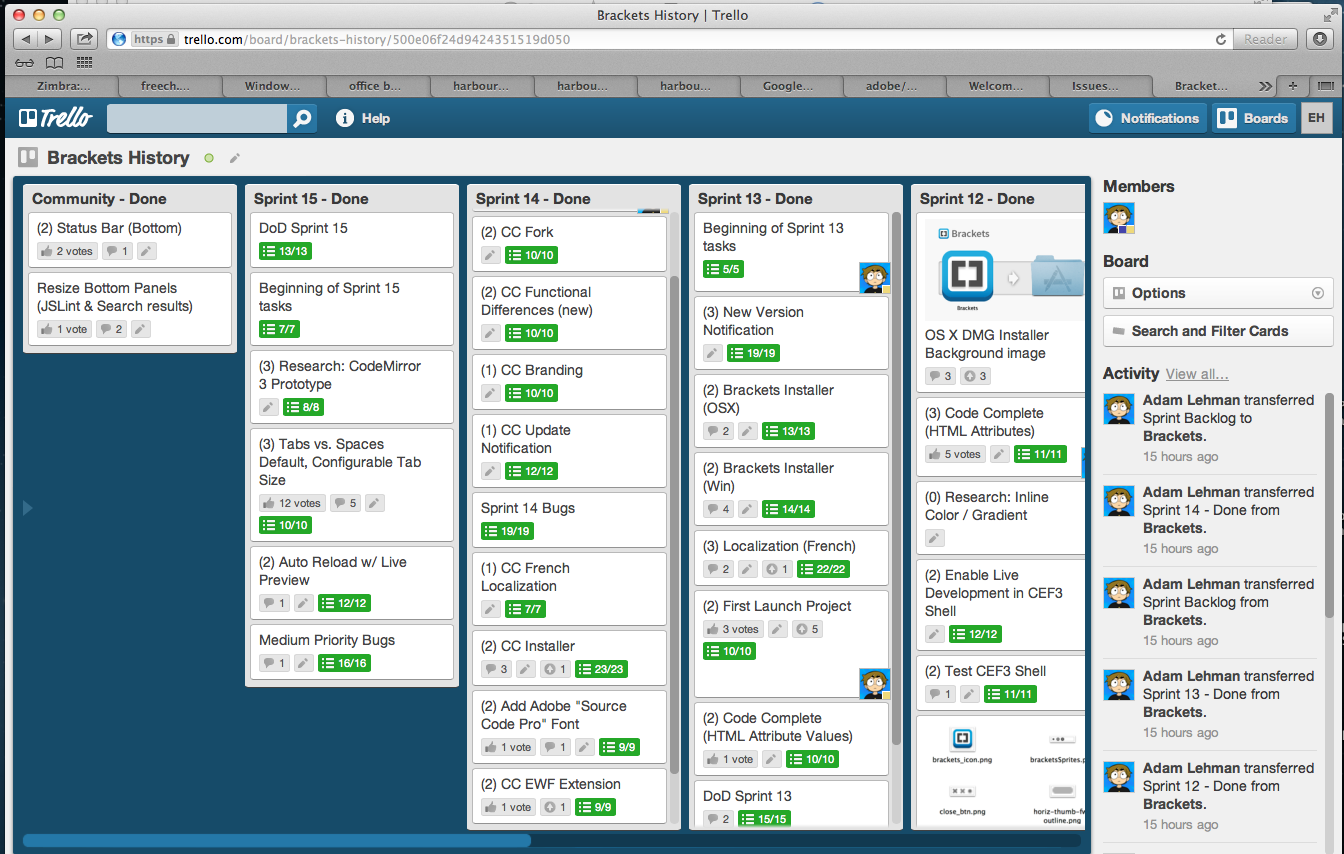
\includegraphics[width=10cm]{img/brackets_trello_sprint_history.png}
\caption{trello}
\end{figure}

\section{Slack}

Slack - "među-story" prostor\citep[str. 275]{agileart}

\section{Estimating}

Velocity, points,  Consistent Estimates

\subsection{Timeboxing, Iteration Timebox}

\section{Commitment}


\chapter{Komunikacija}

\section{Meetings}



TODO

\section{\emph{Issue management} (ISSUE)}

Zadatak, Aktivnost, ticket

''Issue''\footnote{developeri često koriste termin ''ticket'', ili ''bug'' (čak i kada se ne radi o programskog grešci)} predstavlja određeni kokretni projektni zadatak:
\begin{itemize}
  \item prijedlog za realizaciju (ideja)
  \item prijava programske greške (eng. bug)
  \item realizacija nove ili nadogradnja postojeće funkcije sistema (eng. new feature, feature upgrade)
\end{itemize}

\subsection{Poznati alati za \emph{issue management}}

\begin{itemize}
  \item gitlab issues\footnote{\citep{agilegit}}
  \item redmine issues\footnote{\url{http://www.redmine.org}, \url{http://redmine.bring.out.ba}}
\end{itemize}

Sve što je relevantno za projekat treba publikovati na ISSUE sitem.

Ako razvojni tim nije kolociran\footnote{Nalazi se i djeluje na jednom mjestu, nije geografski distribuiran} većina komunikacija između članova obavlja se elektronskim putem.

''Issues management'' sistem je po pitanju realizacije konkretnih projektnih zadataka najbolji način komunikacije.\footnote{email kao sredstvo komunikacije u ove svrhe treba izbjegavati. Email komunikacija brzo postaje nepregledna za većinu projektnih zadataka.}

Komunikacija putem ISSUE sistema time obuhvata komunikaciju na temu novih ideja i prijedloga, realizacije ili nadogradnje funkcija sistema, kao i prijavu i otklanjanje programskih ''bug''-ova (grešaka).

Parcijalni pristup (npr. ograničite se samo na ''bug''-ove) stvara prostor da bitne informacije budu nedostupne svim članovima tima.

Redovno nakon gornje preporuke slijedi pitanje:

Kako ću znati da li je nešto relevantno  ili nije ?

Ako ne znaš da li je relevantno - stavi na ''issue''. 

Nije nikakav problem da se na ticketima u početku nalaze suvišne informacije. Problem je kada informacije nedostaju.

Takođe je vrlo bitno da se informacije na sistem publikuju bez kašnjenje, a ne retroaktivno u formi izvještaja.

Mnoge informacije nakon dan ili dva postaju beskorisne.

Issue management treba reflektovanti život i dinamiku projekta.

\subsection{\emph{Issues} i novi član tima}

''Issues'' su sredstvo komunikacije.

Kada se novi član uključi u ekipu, redmine komentari (ili nedostatak komentara) su odličan indikator kompetencija člana.

Iz njih se vrlo brzo dođe do informacija kojim vještinama član raspolaže, koje su njegove profesionalne navike. Na osnovu tih informacija se može djelovati: 
\begin{itemize}
  \item Organizvati fokusiranu edukaciju za novog člana
  \item Zajednički rad sa iskusnijim kolegama itd.
\end{itemize}

\chapter{Inkrementalni dizajn}

\chapter{Development}

\section{\emph{Source code management} (SCM)}

Detaljno u materijalu ''Agilni \emph{software development}, GIT SCM''\citep{agilegit}

\section{Testiranje}

Testiranje i refactoring etaljno u materijalu ''Agilni \emph{software development}, Tehnike testiranja''\citep{agiletest}

\section{Stalna integracija (CI)}

Detaljno u materijalu ''Agilni \emph{software development}, \emph{Continuous Integration} (CI)''\citep{agileci}

\section{\emph{''Jednom i samo jednom''}}

''Jednom i samo jednom'' (eng. ''Once and Only once'') princip:

\begin{quotation}
  Svaki koncept izrazi jednom. (i samo jednom !).\footnote{\citep[str. 319]{agileart}}
\end{quotation}


\section{\emph{Spike} rješenja}

Spike (\href{http://translate.google.com/#en/hr/spike}{\color{blue}{bos. ekser, smeč}}) razjašnjavaju tehička pitanja koje susrećemo, pri čemu se izbjegava kompleksnost produkcijskog k\^oda.\citep[str. 334]{agileart}


\chapter{Release management}

\section{Testno vs produkcijsko okruženje}

Detaljno u materijalu ''Agilni \emph{software development}, \emph{Test} \& \emph{deploy} infrastruktura''\citep{agiletestdeploy}

\chapter{Agilno = haotično ?!}

Striktne granice između faza dizajna, implementacije i isporuke rješenja korisniku nestaju.

Prakticiranjem TDD-a developer stalno mijenja dizajn\footnote{inkrementalni dizajn TODO: referenciraj se na poglavlje} u malim koracima u toku implementacije.

Breakthrough faze obezbjeđuju veće promjene. Bitno je uočiti da se te promjene dešavaju u najbolje, najproduktivnije vrijeme - onda kada developer ''sazrije'' po pitanju konkretnog problema, kada dobro ovlada postojećim stanjem - njegovim ograničenjima i dobrim stranama.

Što ne trebaš (čega nema u \emph{story}-jima) - ne implementiraj !

Nemamo potrebu anticiparti dizajnerska i arhitektonska rješenja na duge staze.

Nedostatak anticipacije će voditi ''siromašnim'', ''kratkovidnim'' rješenjima ?

{\color{red}{::ODGOVORITI, ELABORIRRATI::}}



\chapter{Zaključak}

Agilni \emph{software development} naravno nije \emph{Silver Bullet}\footnote{\url{http://en.wikipedia.org/wiki/No_Silver_Bullet}}

Međutim, on iz temelja mijenja uvriježene inžinjerske prakse. Agilni pristup unosi ''životnost'' u razvojni proces software-a.

U toku razvoja sofware-a\footnote{ali i sveukupnog životnog ciklusa} se od članova razvojnog tima u znak rezignacije mogu čuti konstatacije slijedećeg tipa:
\begin{quotation}
  \emph{Hah, sve bi bilo u redu da živimo u idealnom svijetu ... Da imamo dovoljno vremena i/ili developera ... Da smo prije implementacije ''xyz'' funkcije dobili sve potrebne informacije ...}
\end{quotation}

Agilni pristup kao temeljno polazište uzima realni svijet i realne potrebe korisnika software-a.

On razvojni tim stalno podsjeća i usmjerava da je glavni cilj sofverskog projekta ostvariti vrijednost za \emph{korisnika software}-a.\footnote{Prvi slogan moje firme je bio: \emph{Iskoristite računar}. Međutim, slogan se nije puno koristio. Još gore, firma u svom djelovanju u mnogim segmentima odstupila od principa ovog slogana. Nakon 16 godina, rad na ovoj temi me je podsjetio na taj slogan. Iz ove perspetkive mogu konstatovati da je to bio sjajan slogan. Šteta što smo ga zaboravili - i slovom i djelom.}
Ta vrijednost (upotrebljivost, korisnost) je sama po sebi vremenski \emph{dinamična} kategorija. Agilni \emph{software development} nastoji razvojni ciklus usaglasiti sa tom činjenicom.

% -------------------------------------------------
\bibliography{literatura}
\bibliographystyle{fit}

% -------------------------------------------------
\appendix

\chapter{Software toolset}
\begin{enumerate}
  \item Mac OS X 10.8.2
  \item mvim, vim tekst editor ver 7.3
  \item MacTex (TeX Live 2012)
\end{enumerate}

\chapter{Software repozitoriji}

\begin{itemize}
  \item Agilni developerski environment - \url{https://github.com/hernad/agile\_dev\_env}

\end{itemize}

\end{document}
